%        File: slides.tex
%     Created: Sab Apr 22 12:00 pm 2017 C
% Last Change: Sab Apr 22 12:00 pm 2017 C
%
\documentclass[10pt]{beamer}
\usepackage[english]{babel}
\usepackage{subfigure}
\usepackage[T1]{fontenc}
\usepackage{microtype}
\usepackage{booktabs}
\usepackage{multirow}
%\usepackage{hyperref}
\usepackage{tikz}
\usepackage{pgfplots}
\usetikzlibrary{arrows,shapes,backgrounds}
\usepackage{adjustbox}
%\usepackage[mode=buildnew]{standalone}
\usepackage[absolute,overlay]{textpos}
\usepackage{xcolor}
\usepackage[version=4]{mhchem}
%\usepackage{listings}
%\lstset{language=C++}
%\lstset{
%		basicstyle=\small\ttfamily,
%		keywordstyle=\color{blue}\bfseries,
%		commentstyle=\color{darkgray},
%		stringstyle=\color{orange}
%		}
% define
\definecolor{mDarkBrown}{HTML}{604c38}
\definecolor{mDarkTeal}{HTML}{23373b}
\definecolor{mLightBrown}{HTML}{EB811B}
\definecolor{mLightGreen}{HTML}{14B03D}
\definecolor{mBackground}{HTML}{FFFFFF}
\renewcommand{\epsilon}{\varepsilon}
\renewcommand{\theta}{\vartheta}
\renewcommand{\rho}{\varrho}
\renewcommand{\phi}{\varphi}
\newcommand{\aof}{\mathring{a}_\text{of}^{(3)}}
\newcommand{\nbb}{\nu\beta\beta}
%\includeonlyframes{current}
% metropolis theme options
\usetheme[numbering=fraction, sectionpage=none, subsectionpage=progressbar]{metropolis}
\usepackage{appendixnumberbeamer}
\setbeamercolor{background canvas}{bg=white}
\setbeamercovered{dynamic}
\title{A test for Lorentz and CPT invariance from the double-beta decay energy spectrum \\ \small{Work in progress\ldots}}
\titlegraphic{\vspace{4.8cm}\begin{flushright}
\includegraphics[width=1.8cm]{img/infn-logo.png}\hspace{5mm}
\includegraphics[width=1.8cm]{../img/logo.pdf}\end{flushright}}
\date{April 27, 2017}
\author{Luigi Pertoldi}
\institute{Università degli Studi di Padova \\ INFN - Sezione di Padova}
%
\begin{document}
\maketitle
%\begin{frame}{Index}
%	\setbeamertemplate{section in toc}[sections numbered]
%	\tableofcontents%[hideallsubsections]
%\end{frame}
\begin{frame}{Beyond the Standard Model}
	\begin{itemize}
		\item The Spontaneous Symmetry Breaking (SSB) of the Lorentz symmetry can be accomodated by many candidate theories of quantum gravity (e.g. string theory). The general framework to study this kind of phenomena is the \textcolor{mLightGreen}{Standard Model Extension (SME)}.
		\item Direct studies of physics at the Planck scale are currently impossible, however we can look for suppressed signals at the energy scales we can access today.
		\item This kind of SSB can be tested in neutrino experiments involving:
		\begin{itemize}
			\item oscillations
			\item time-of-flight measurements
			\item \textcolor{mLightBrown}{neutrino's phase space properties $\rightarrow$ decays}
		\end{itemize}
	\end{itemize}
\end{frame}
\begin{frame}{The energy spectrum of $2\nbb$}
	\begin{columns}
		\column{0.5\textwidth}
			\metroset{block=fill}
			\begin{exampleblock}{Standard Model $2\nbb$}
			\[\begin{split}
				\frac{d\Gamma}{dK} &=C(K^5+10K^4+40K^3+ \\
				&+60K^2+30){\color{blue}(K_0-K)^5}
			\end{split}\]
			\end{exampleblock}
			\begin{exampleblock}{Lorentz Violating $2\nbb$}
			\[\begin{split}
				\frac{d\Gamma}{dK} &=C(K^5+10K^4+40K^3+ \\
				&+60K^2+30){\color{red}10\aof(K_0-K)^4}
			\end{split}\]
			\end{exampleblock}
		\column{0.5\textwidth}
			\vspace{1cm}
			\begin{center}
				\begin{adjustbox}{scale=1.2}
				\begin{tikzpicture}
					\begin{axis}[
								mlineplot,
								width=\textwidth, height=6cm,
								xmin=0, xmax=4.5,
								ymin=0, ymax=0.6,
								samples=200,
								xlabel=Energy/$m_e$,
								yticklabels={,,}
								ylabel=a.u.
								]
						\addplot [mark=none, color=red, line width=1pt, domain=0:4] 
							{x*(4-x)^4*((x)^4+10*(x)^3+40*(x)^2+60*(x)+30)/27814};
						\addplot [mark=none, color=blue, line width=1pt, domain=0:4] 
							{x*(4-x)^5*((x)^4+10*(x)^3+40*(x)^2+60*(x)+30)/65749};
						%\node[pin=30:{$2\nu\beta\beta$}] at (axis cs:2,2.3) {};
						%\addplot [mark=none, color=blue, line width=1pt, domain=4:5] {0};
						%\node[pin=90:{$0\nu\beta\beta$}] at (axis cs:4,0.8) {};
					\end{axis}
				\end{tikzpicture}
				\end{adjustbox}
			\end{center}
	\end{columns}
\end{frame}
\begin{frame}
	\metroset{block=fill}
	\begin{alertblock}{Target}
		Extract an upper limit for $\aof$ using data from \texttt{PhaseII} with a Bayesian Analysis (\texttt{BAT} package)
	\end{alertblock}
	\begin{itemize}
	\item Data from \alert{\texttt{tier3}} are used (no PSD, no LAr veto). \\ Runs \texttt{53-74}, excluding \texttt{66} and \texttt{68}.
	\item Spectra from \texttt{BEGe}s (excluding \texttt{GD02D}) and from enriched coaxials are simultaneously fitted
	\item A \alert{variable binning} is adopted to take into account the energy resolution: bins (4 keV) containing $\gamma$ lines are merged into one.
	\item \alert{Background model:} Up to now the presence of $\ce{^{212}Bi}$, $\ce{^{214}Bi}$, $\ce{^{208}Tl}$, $\ce{^{214}Pb}$, $\ce{^{40}K}$, $\ce{^{42}K}$, $\ce{^{60}Co}$, $\ce{^{228}Ac}$ and $\ce{^{234}Pa}$ has been tested in different components of the experimental apparatus (work in progress\ldots)
	\end{itemize}
\end{frame}
\begin{frame}{Fit results --- [570 keV, 1800 keV]}
	\centering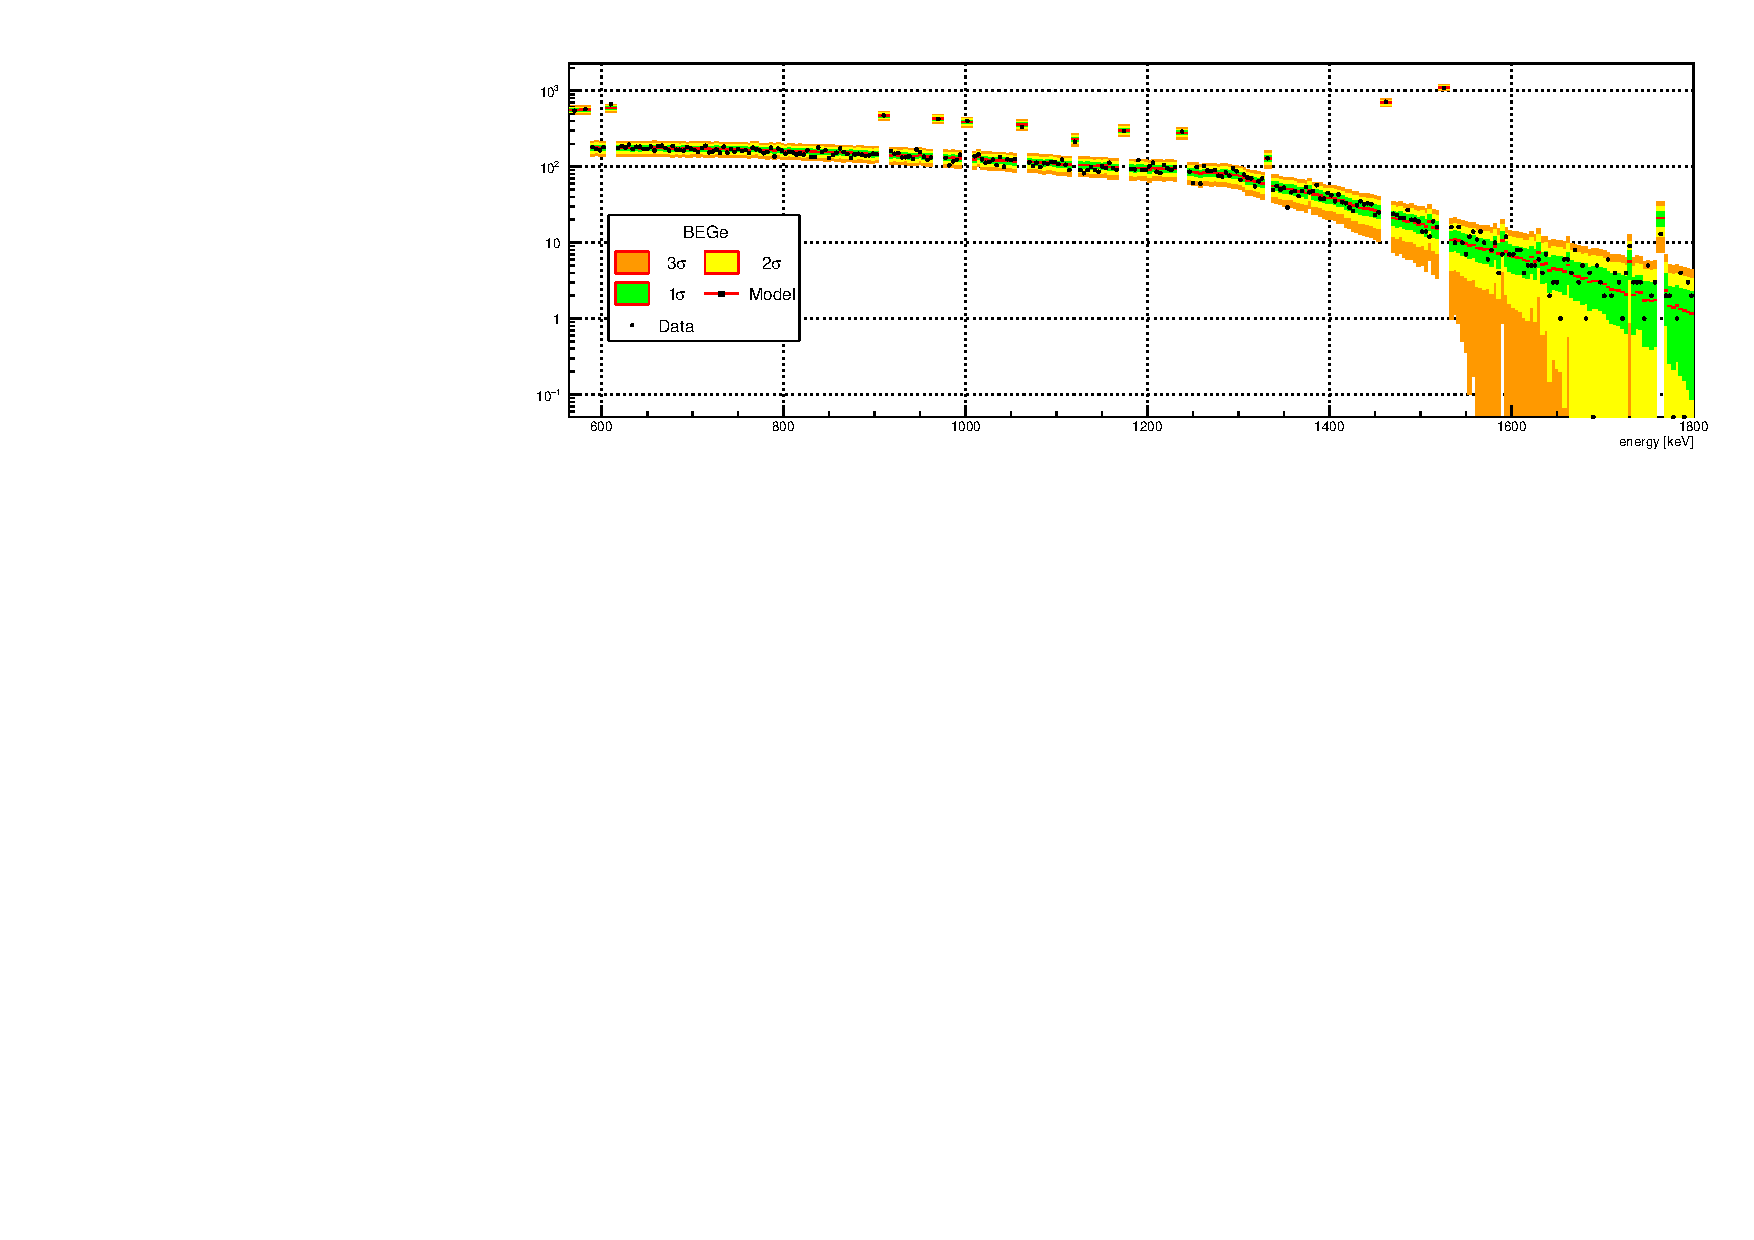
\includegraphics[height=\textwidth, angle=270]{img/BEGe.pdf} \\
	\centering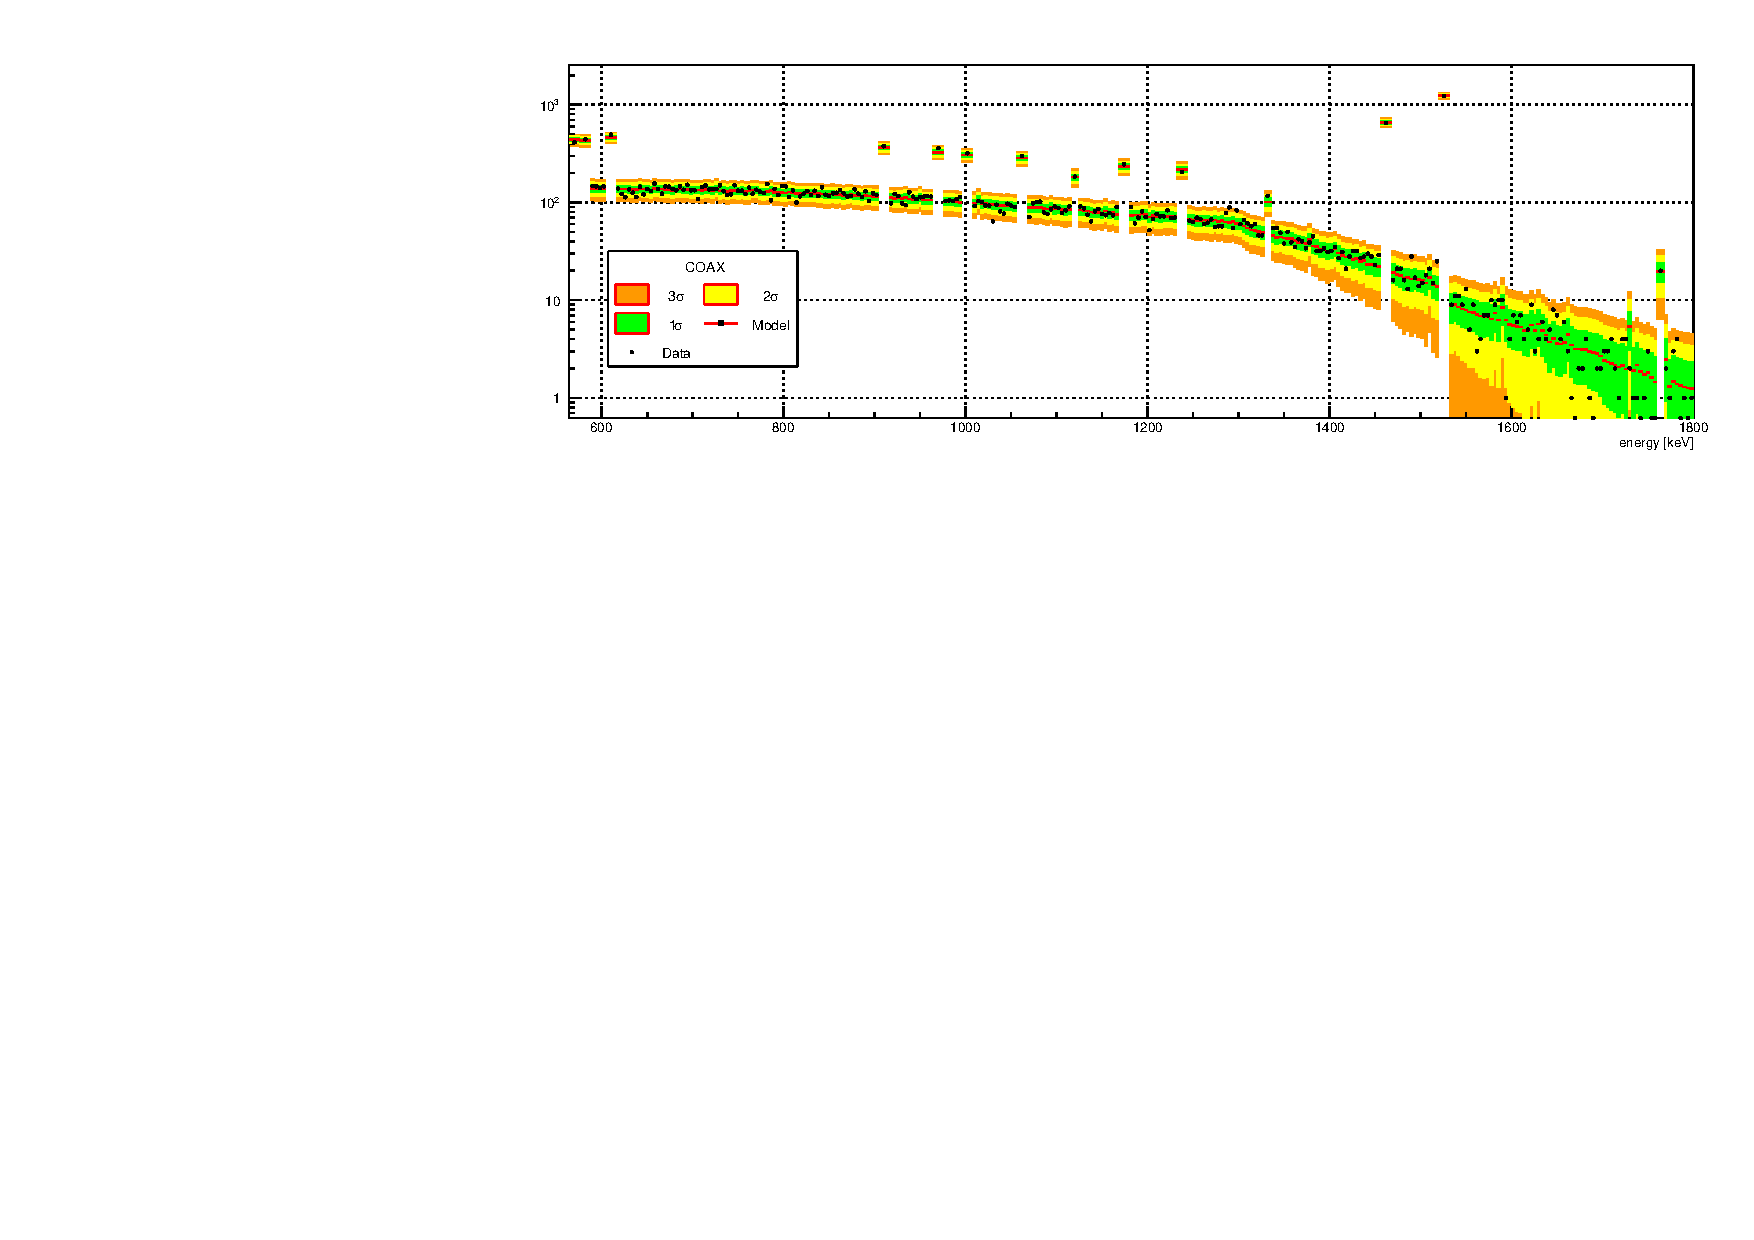
\includegraphics[height=\textwidth, angle=270]{img/COAX.pdf}
\end{frame}
\begin{frame}{Fit results --- [1800 keV, 5300 keV]}
	\centering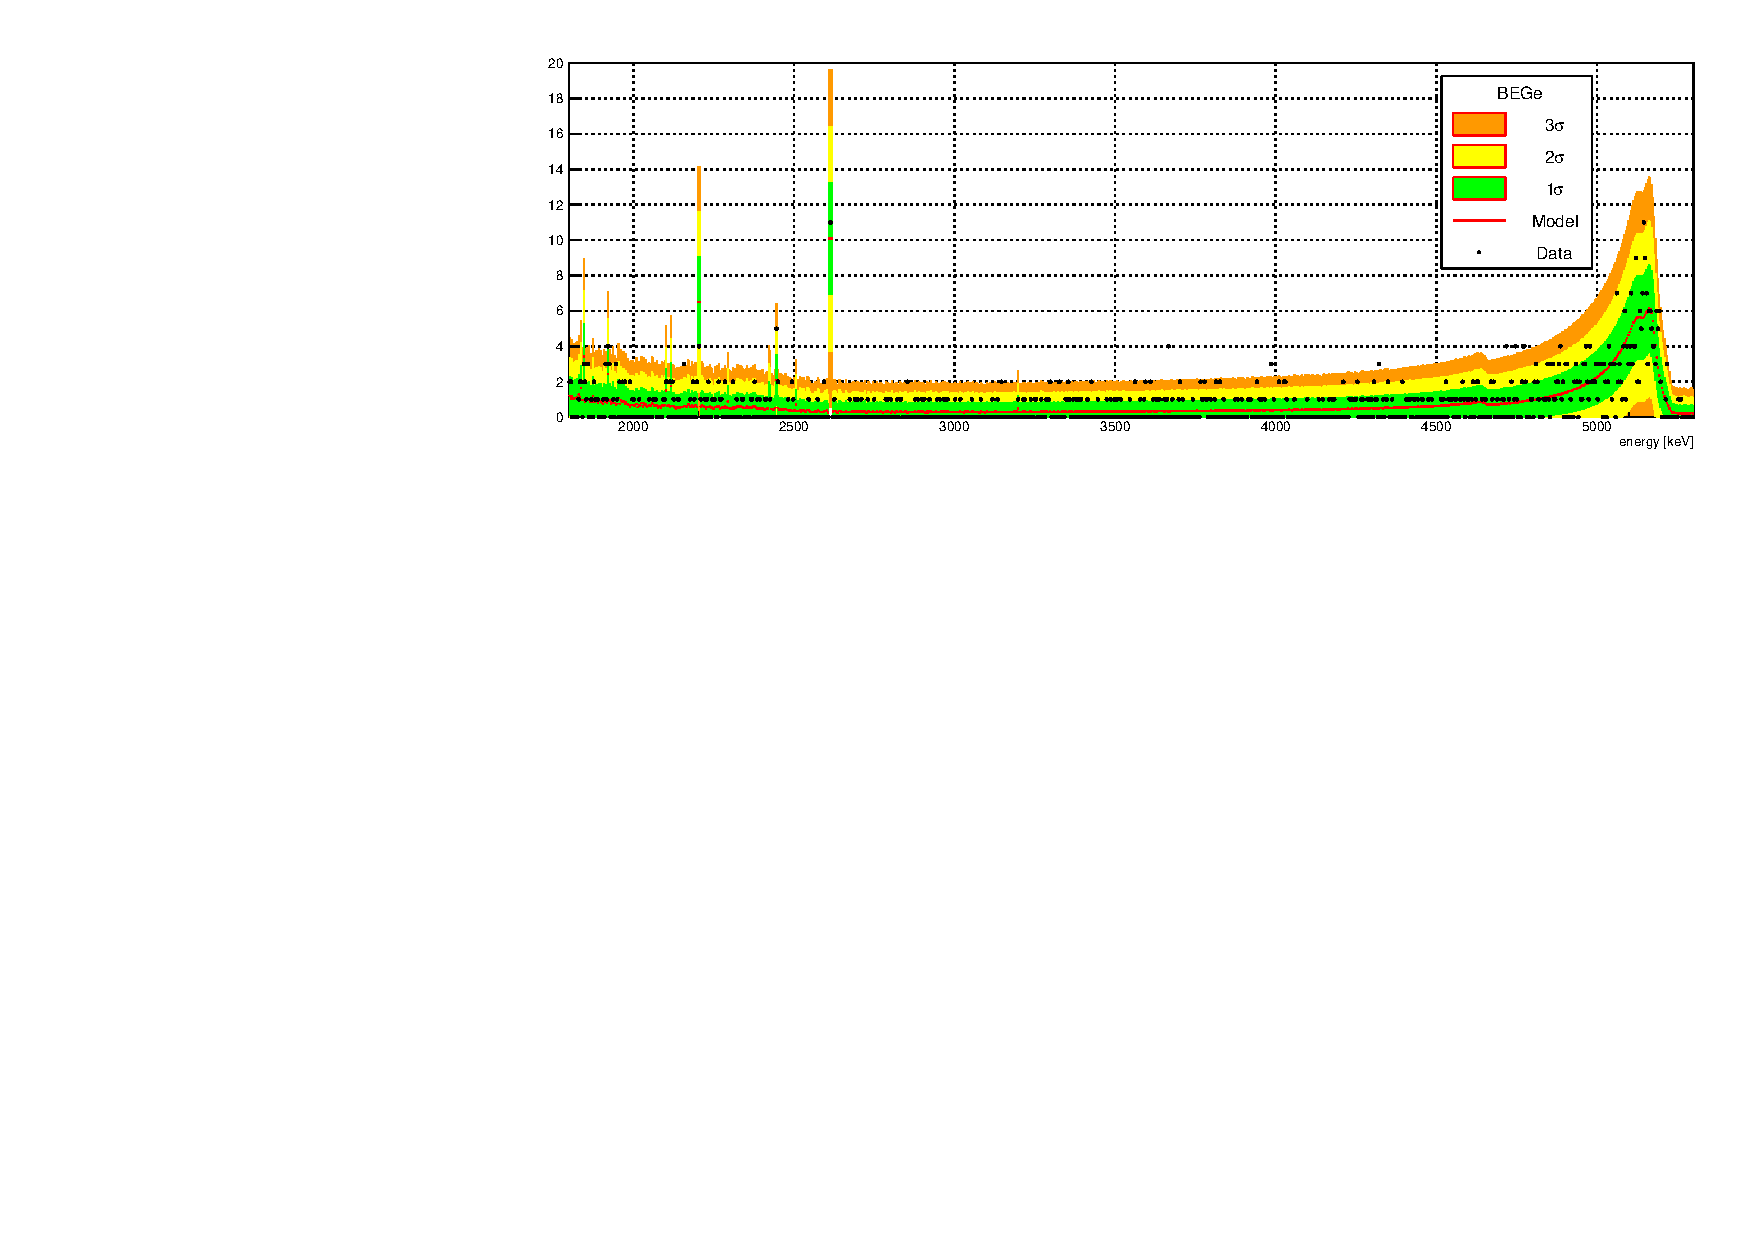
\includegraphics[height=\textwidth, angle=270]{img/BEGealpha.pdf} \\
	\centering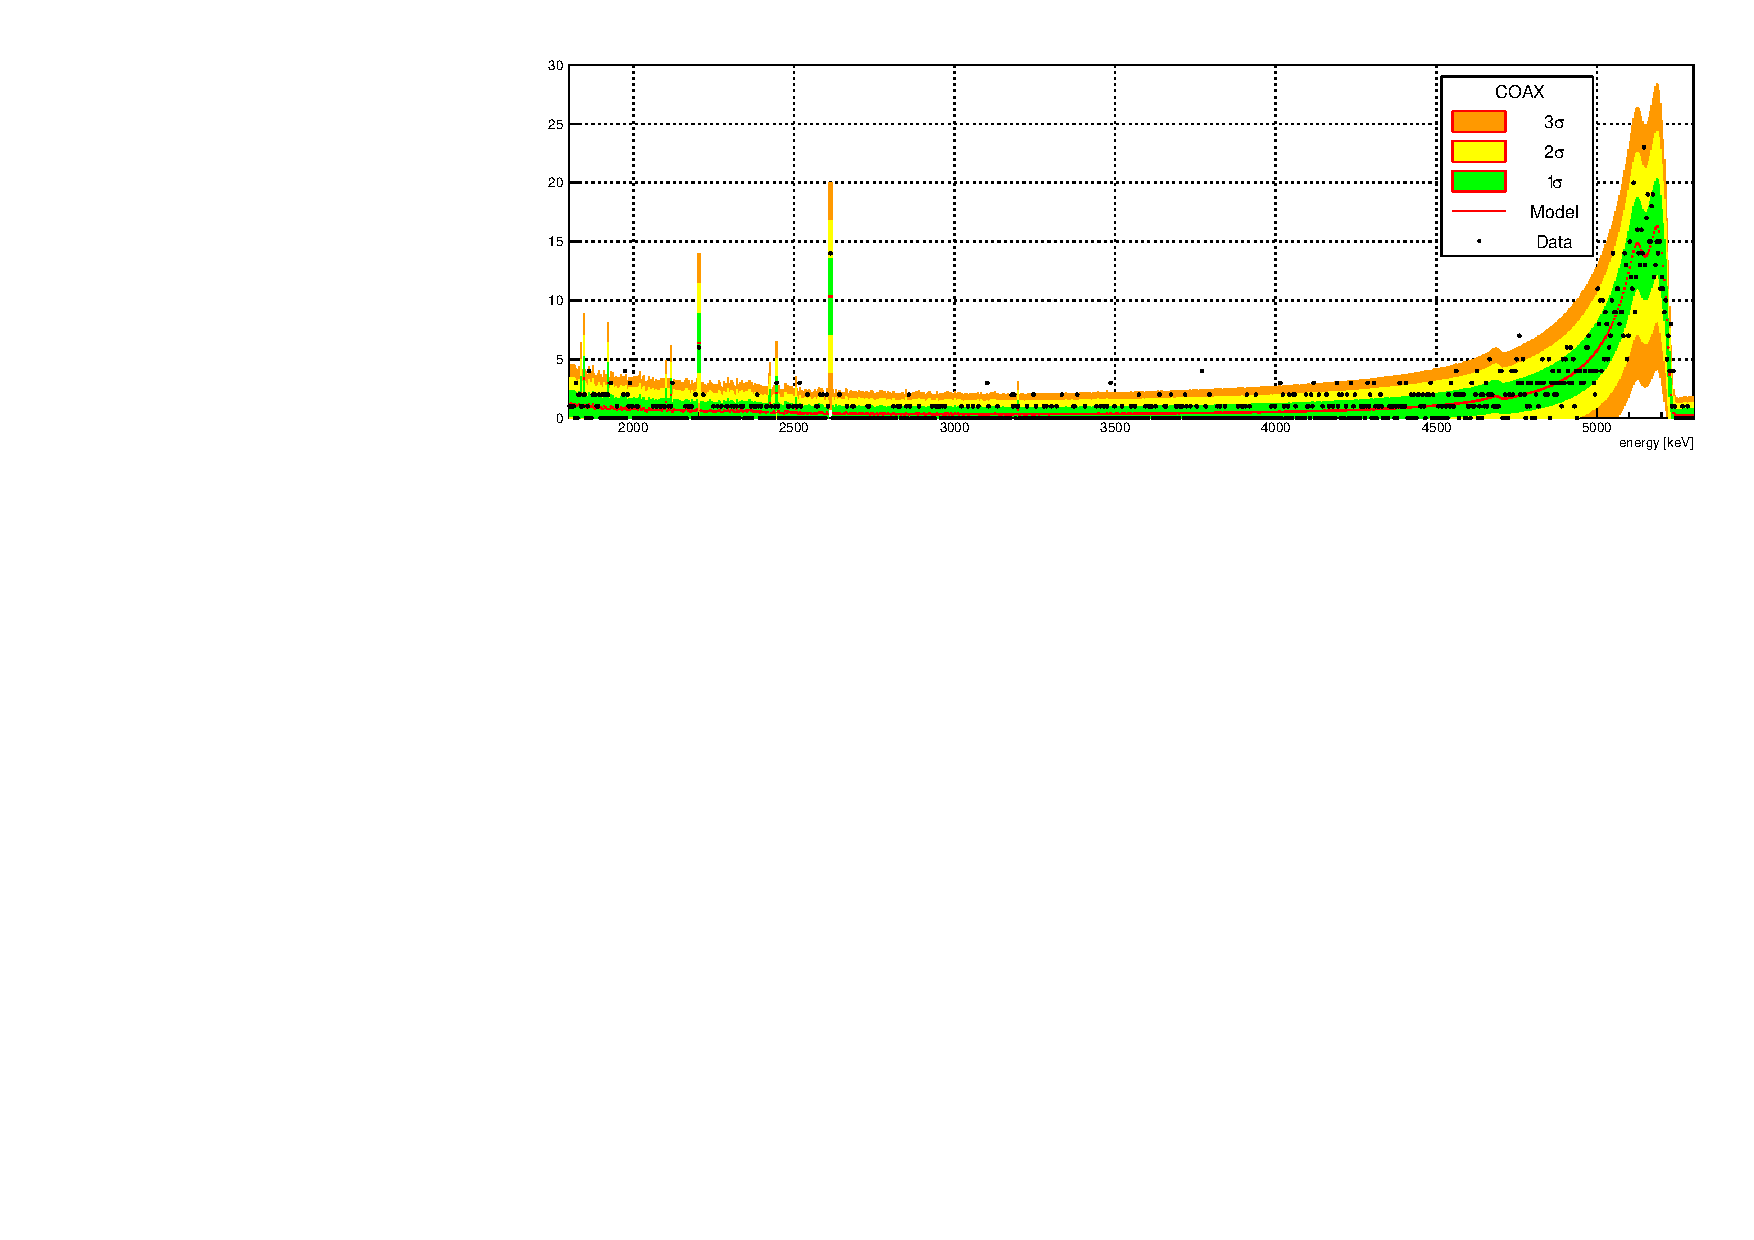
\includegraphics[height=\textwidth, angle=270]{img/COAXalpha.pdf}
\end{frame}
\begin{frame}{Background sources --- [570 keV, 1800 keV]}
	\centering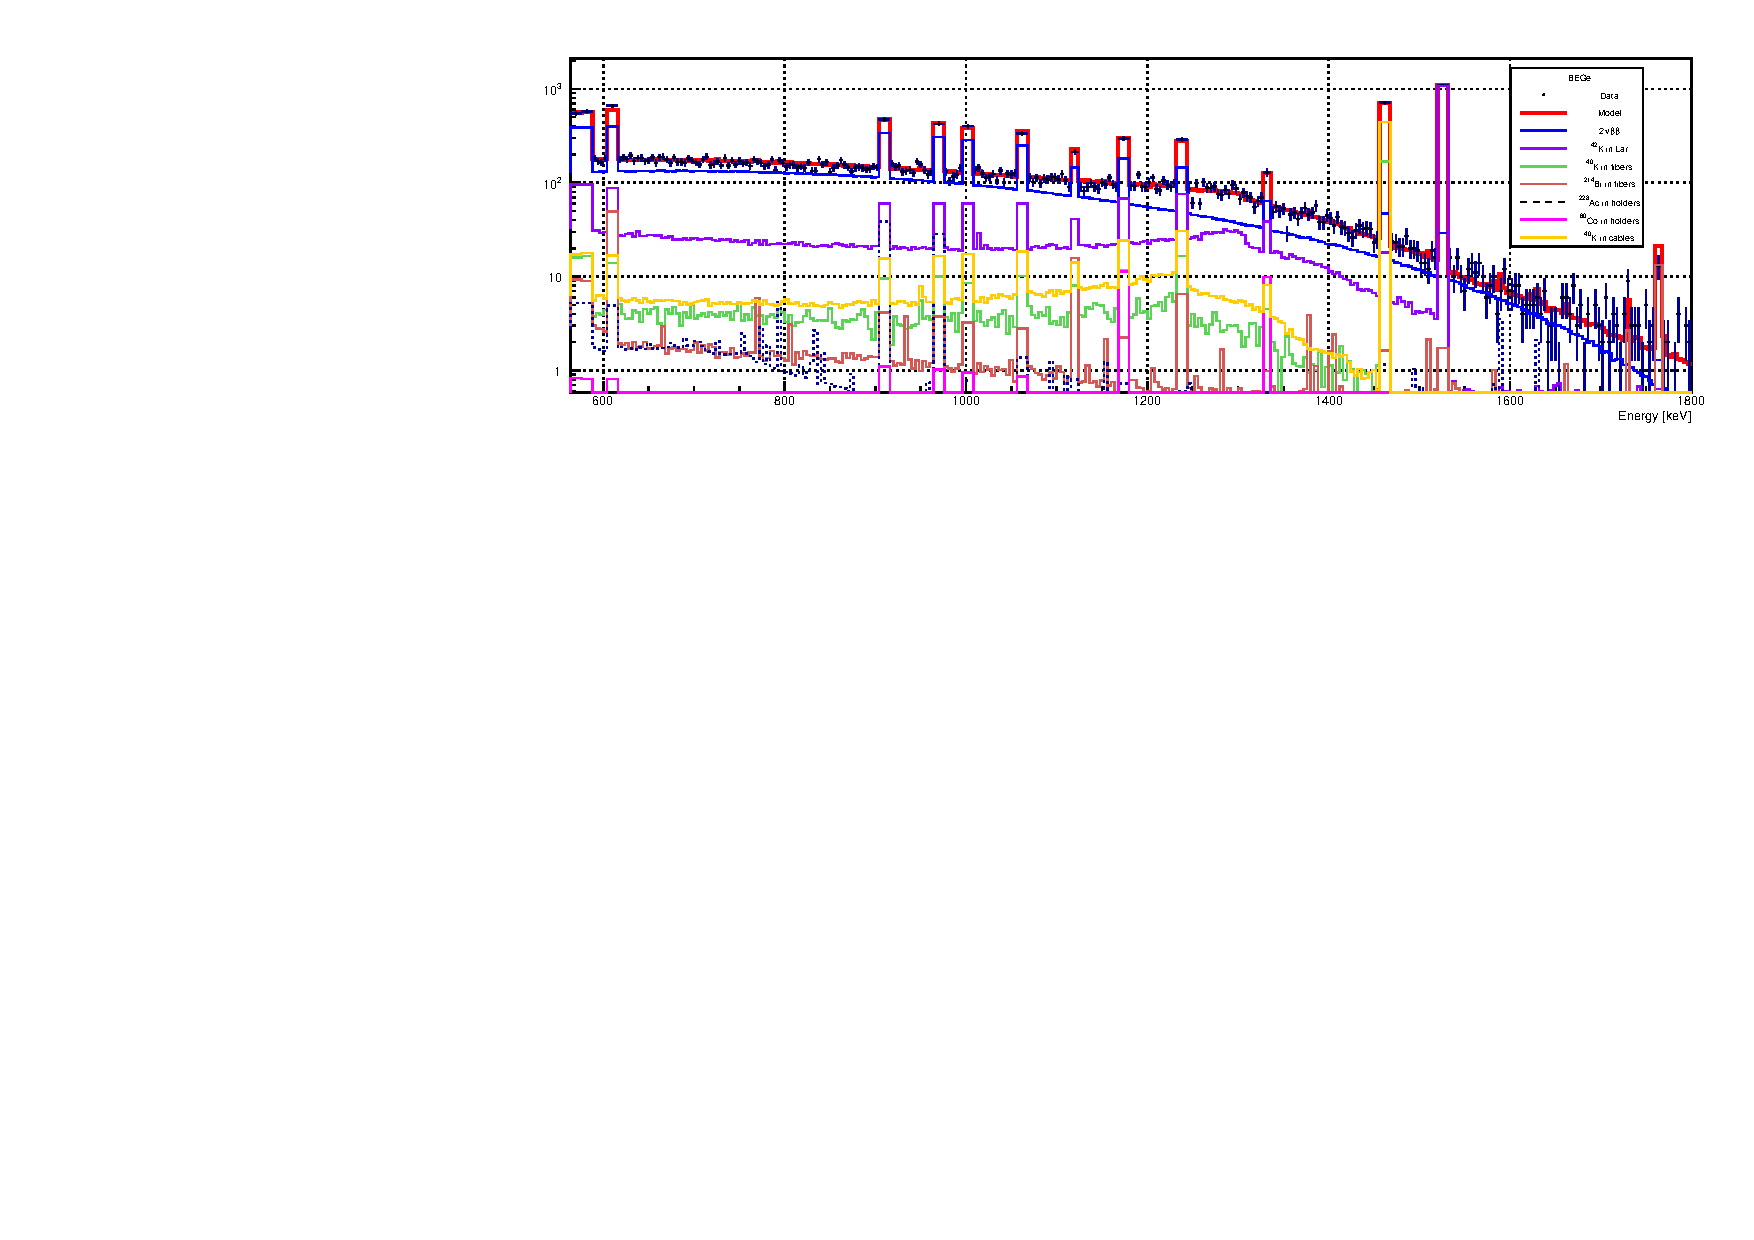
\includegraphics[height=\textwidth, angle=270]{img/bkgBEGe.pdf} \\
	\centering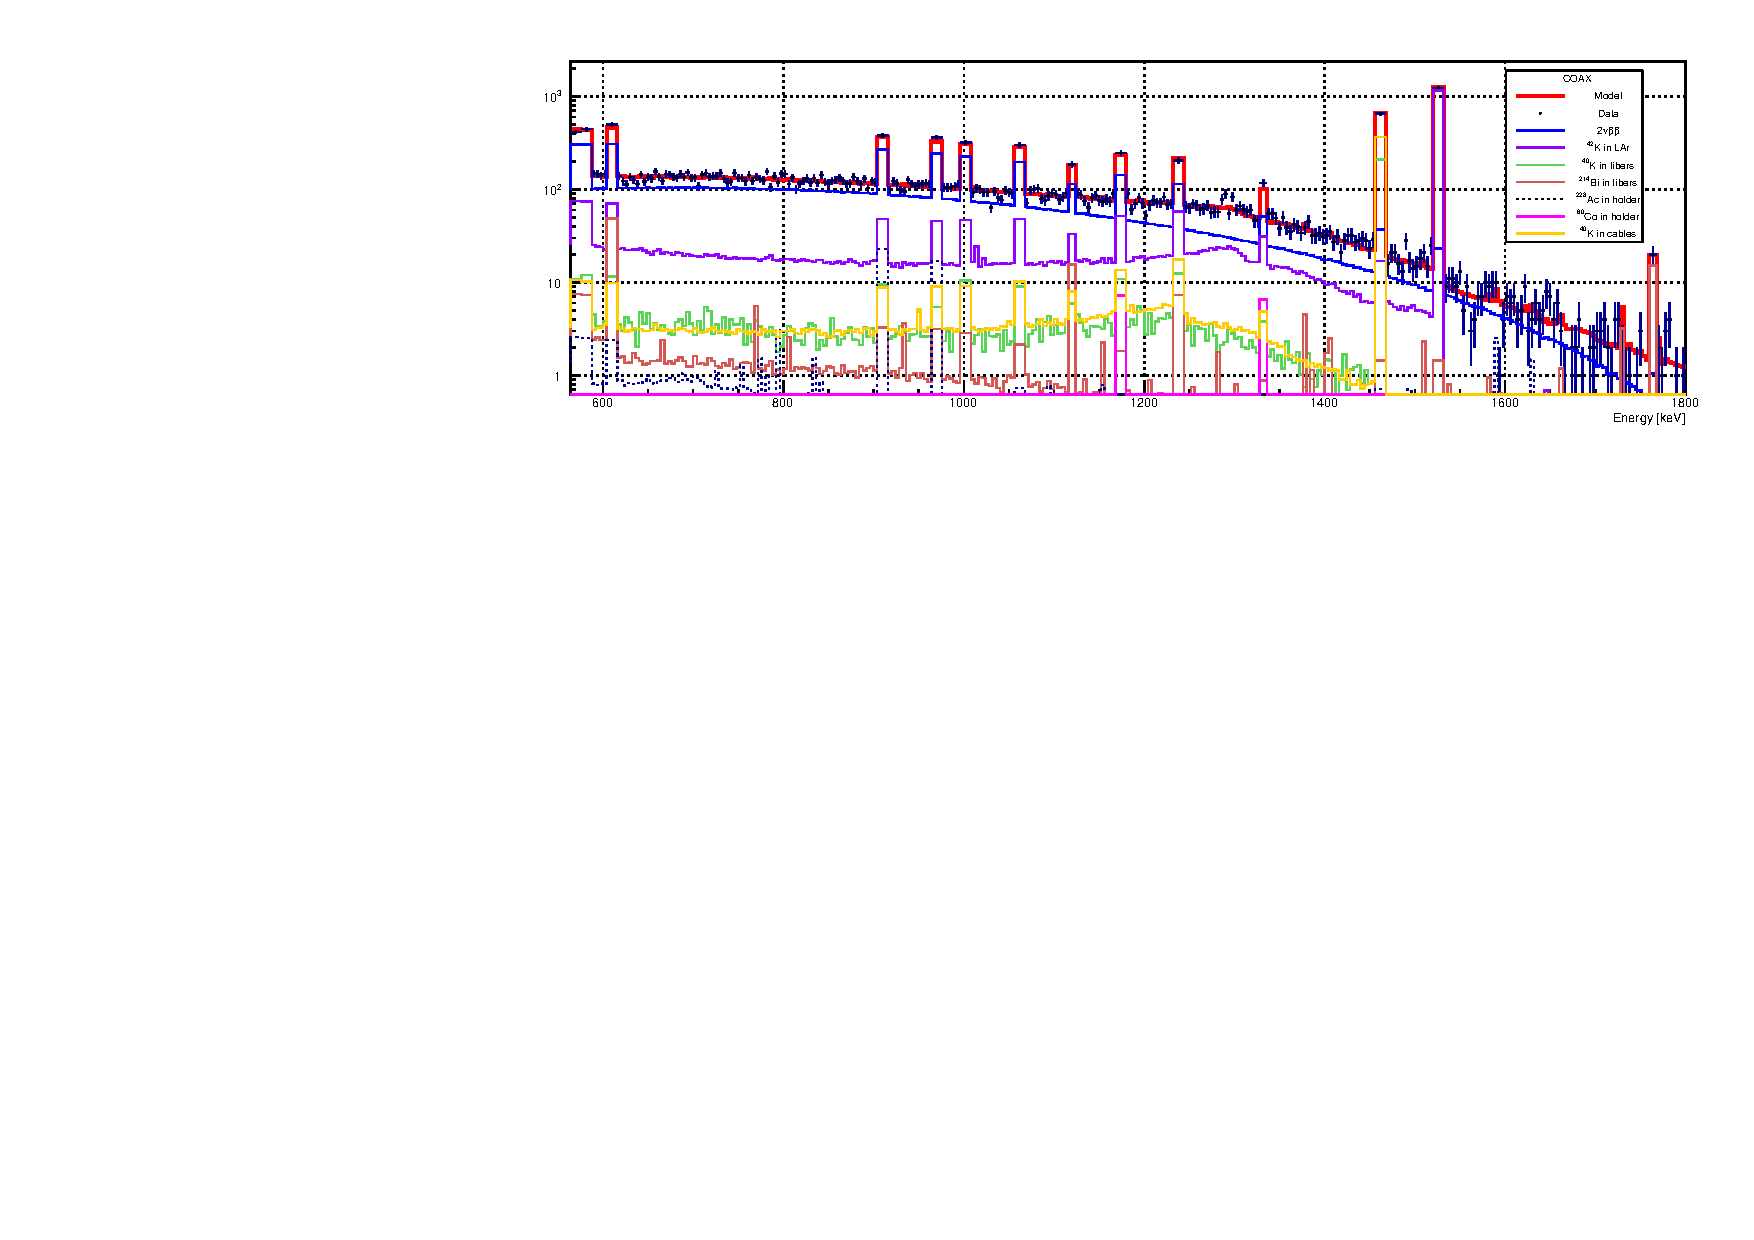
\includegraphics[height=\textwidth, angle=270]{img/bkgCOAX.pdf}
\end{frame}
\begin{frame}{Background sources --- [1800 keV, 2200 keV]}
	\centering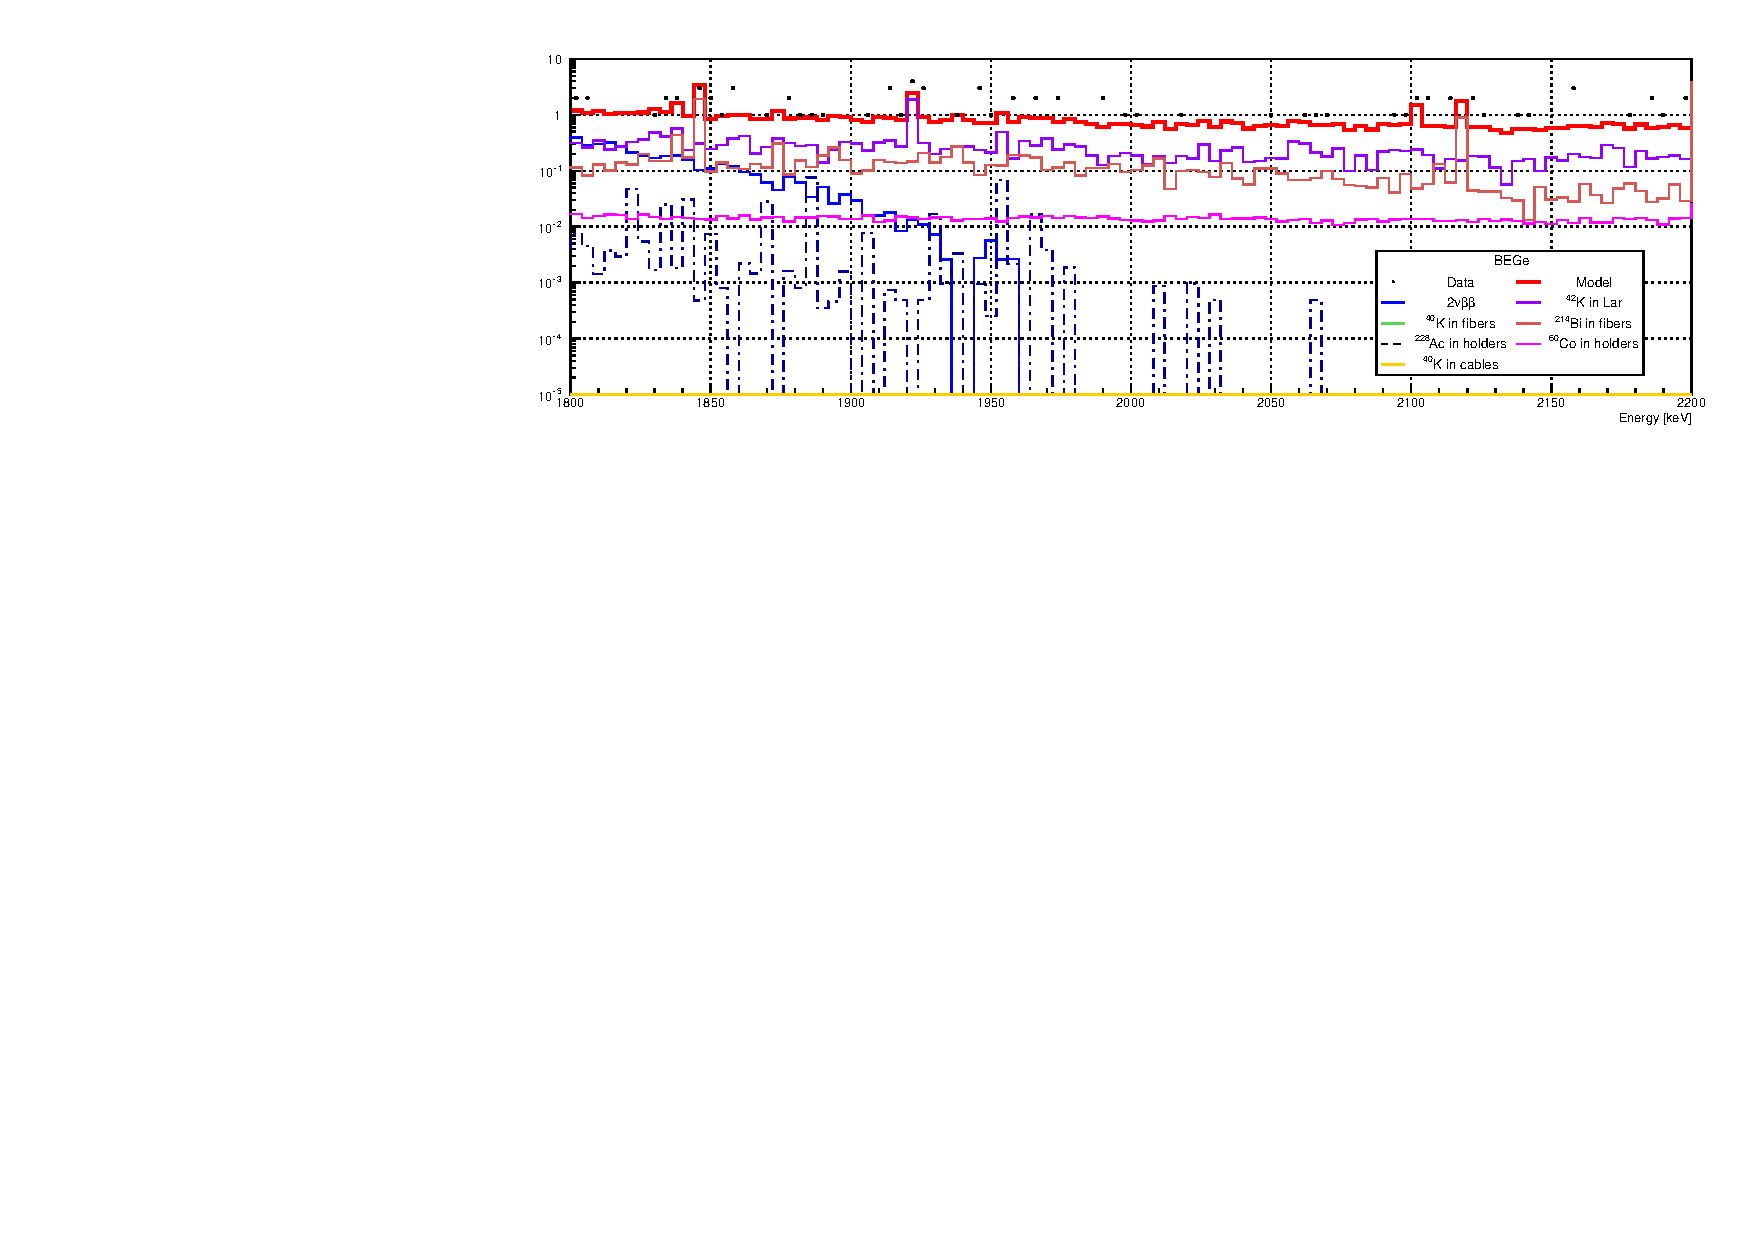
\includegraphics[height=\textwidth, angle=270]{img/bkgBEGeroi.pdf} \\
	\centering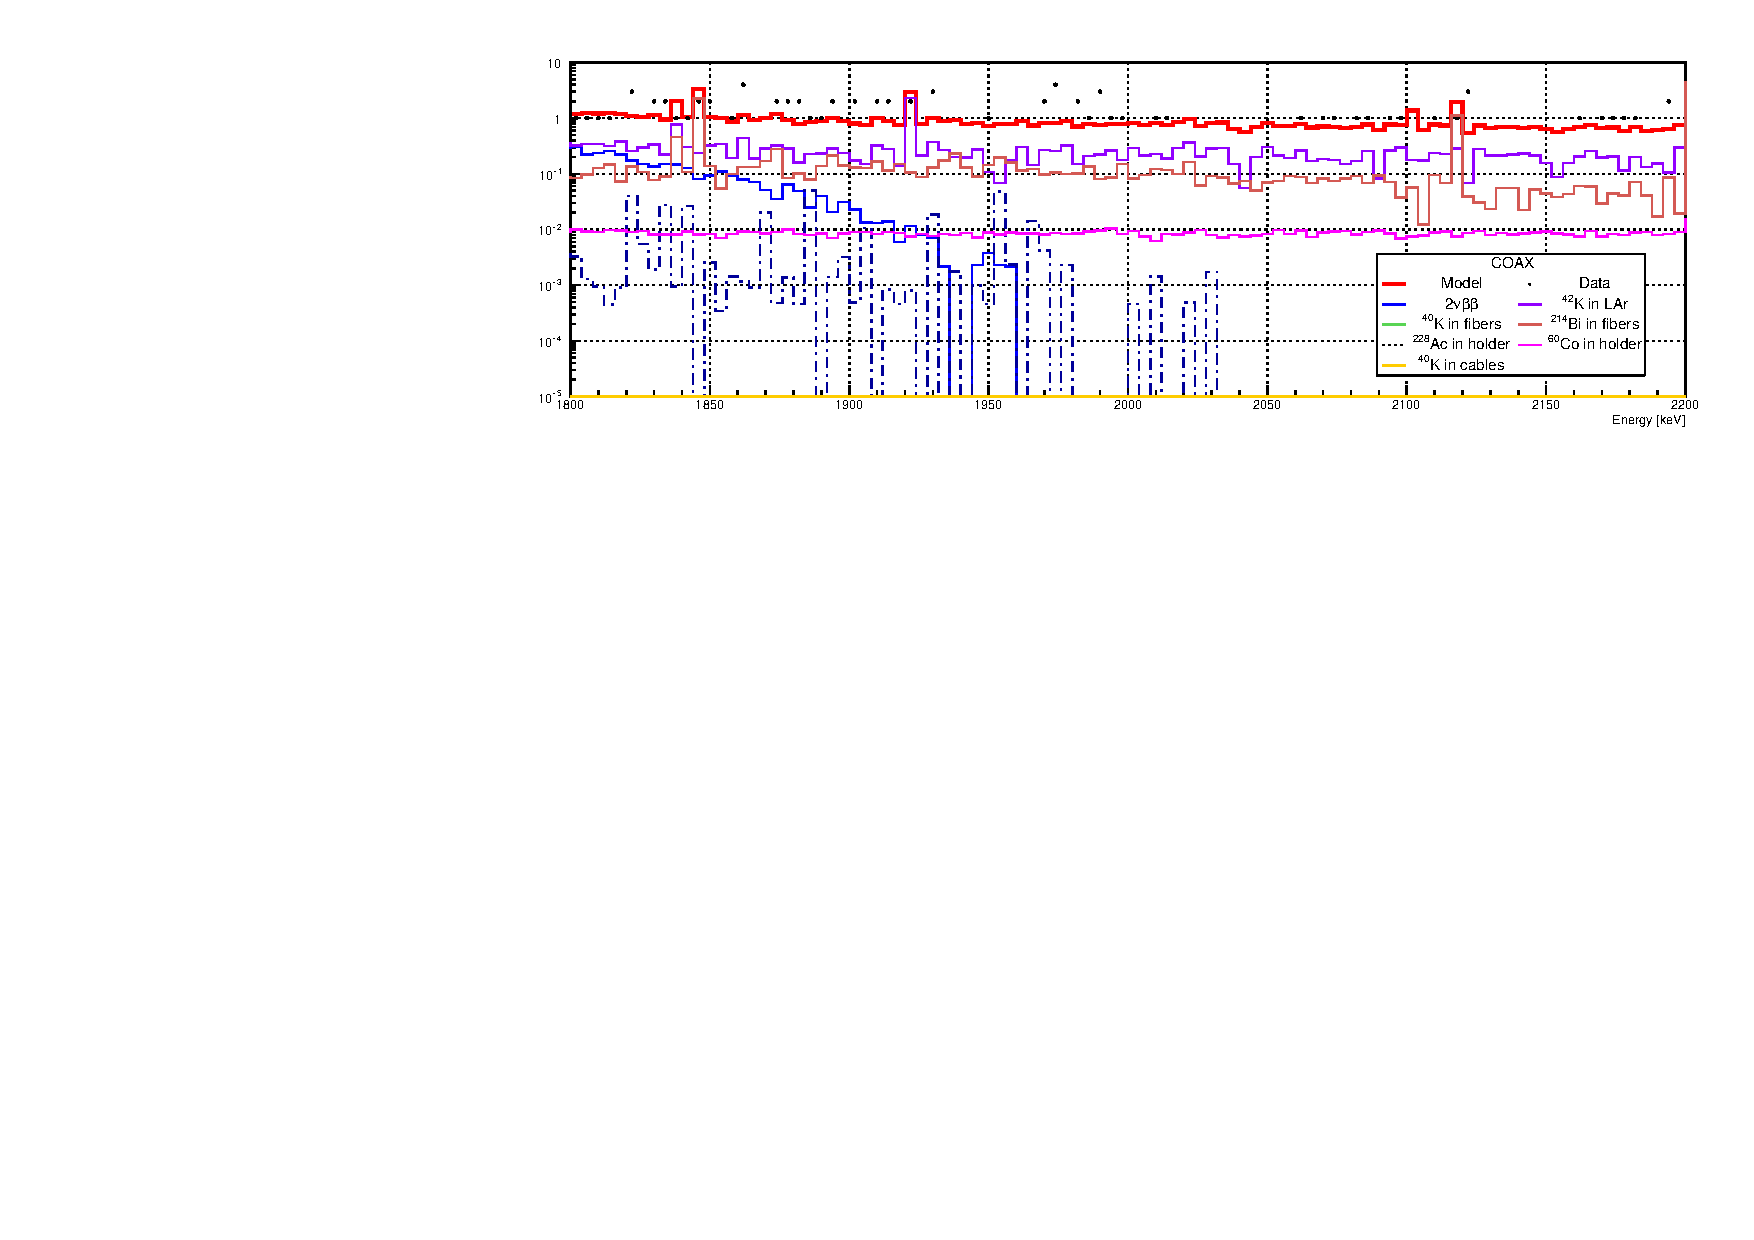
\includegraphics[height=\textwidth, angle=270]{img/bkgCOAXroi.pdf}
\end{frame}
\begin{frame}{Residuals --- [570 keV, 1800 keV]}
	\centering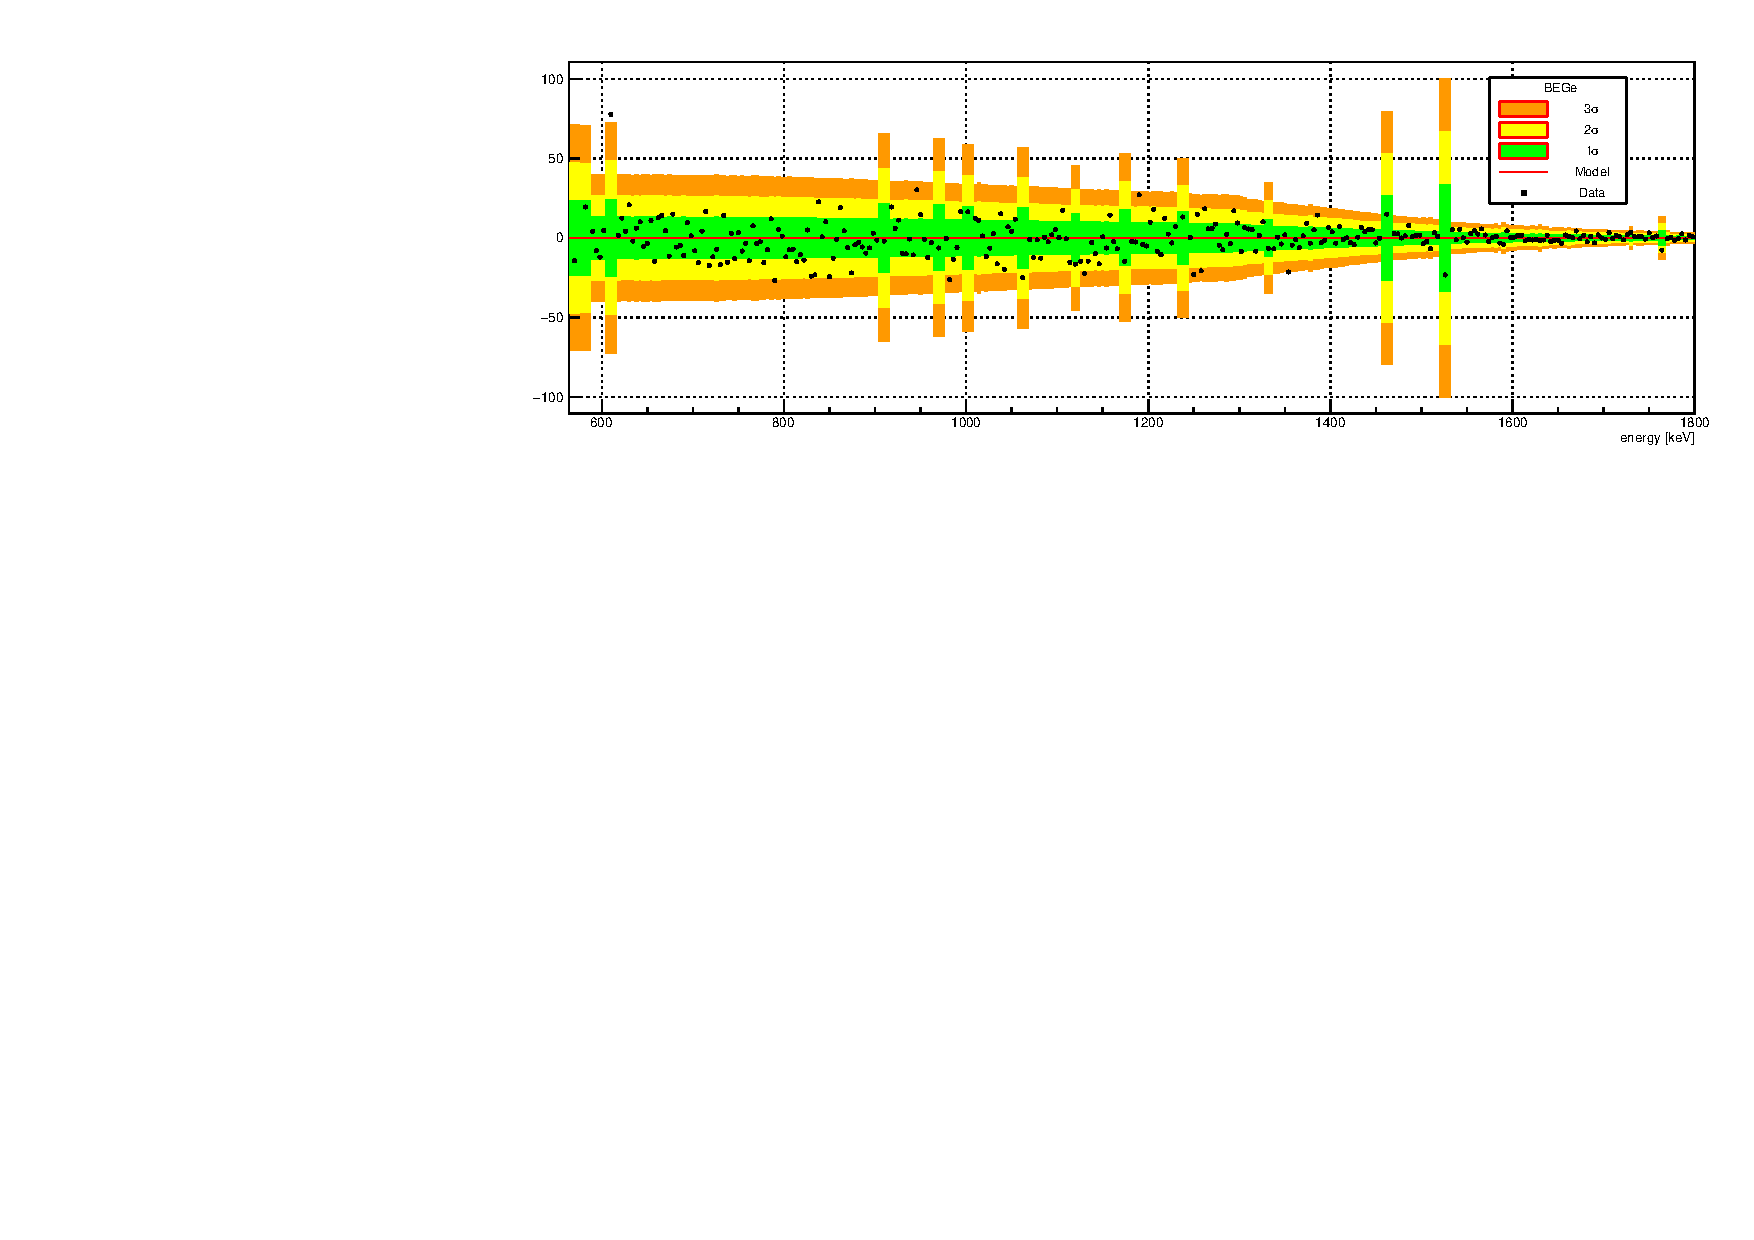
\includegraphics[height=\textwidth, angle=270]{img/resBEGe.pdf} \\
	\centering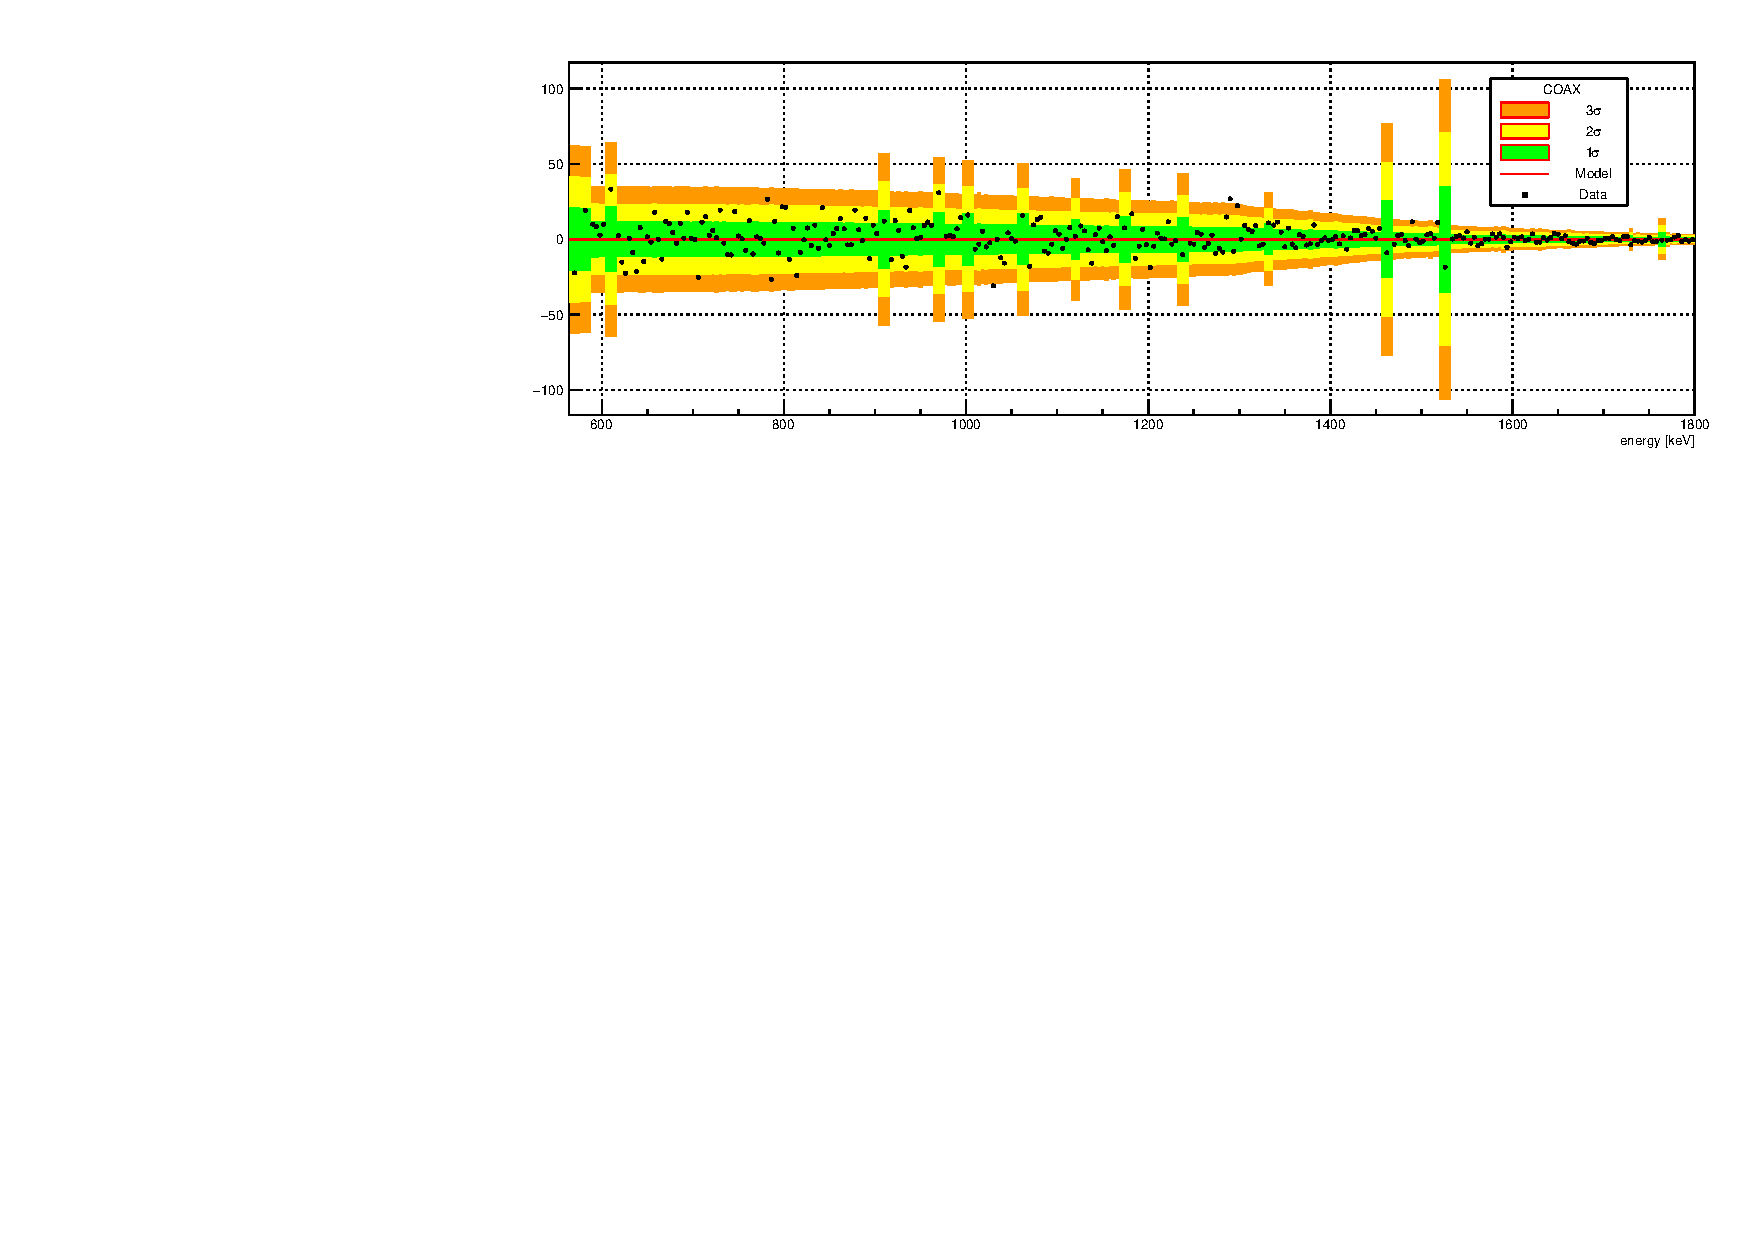
\includegraphics[height=\textwidth, angle=270]{img/resCOAX.pdf}
\end{frame}
\begin{frame}{Residuals --- [1800 keV, 5300 keV]}
	\centering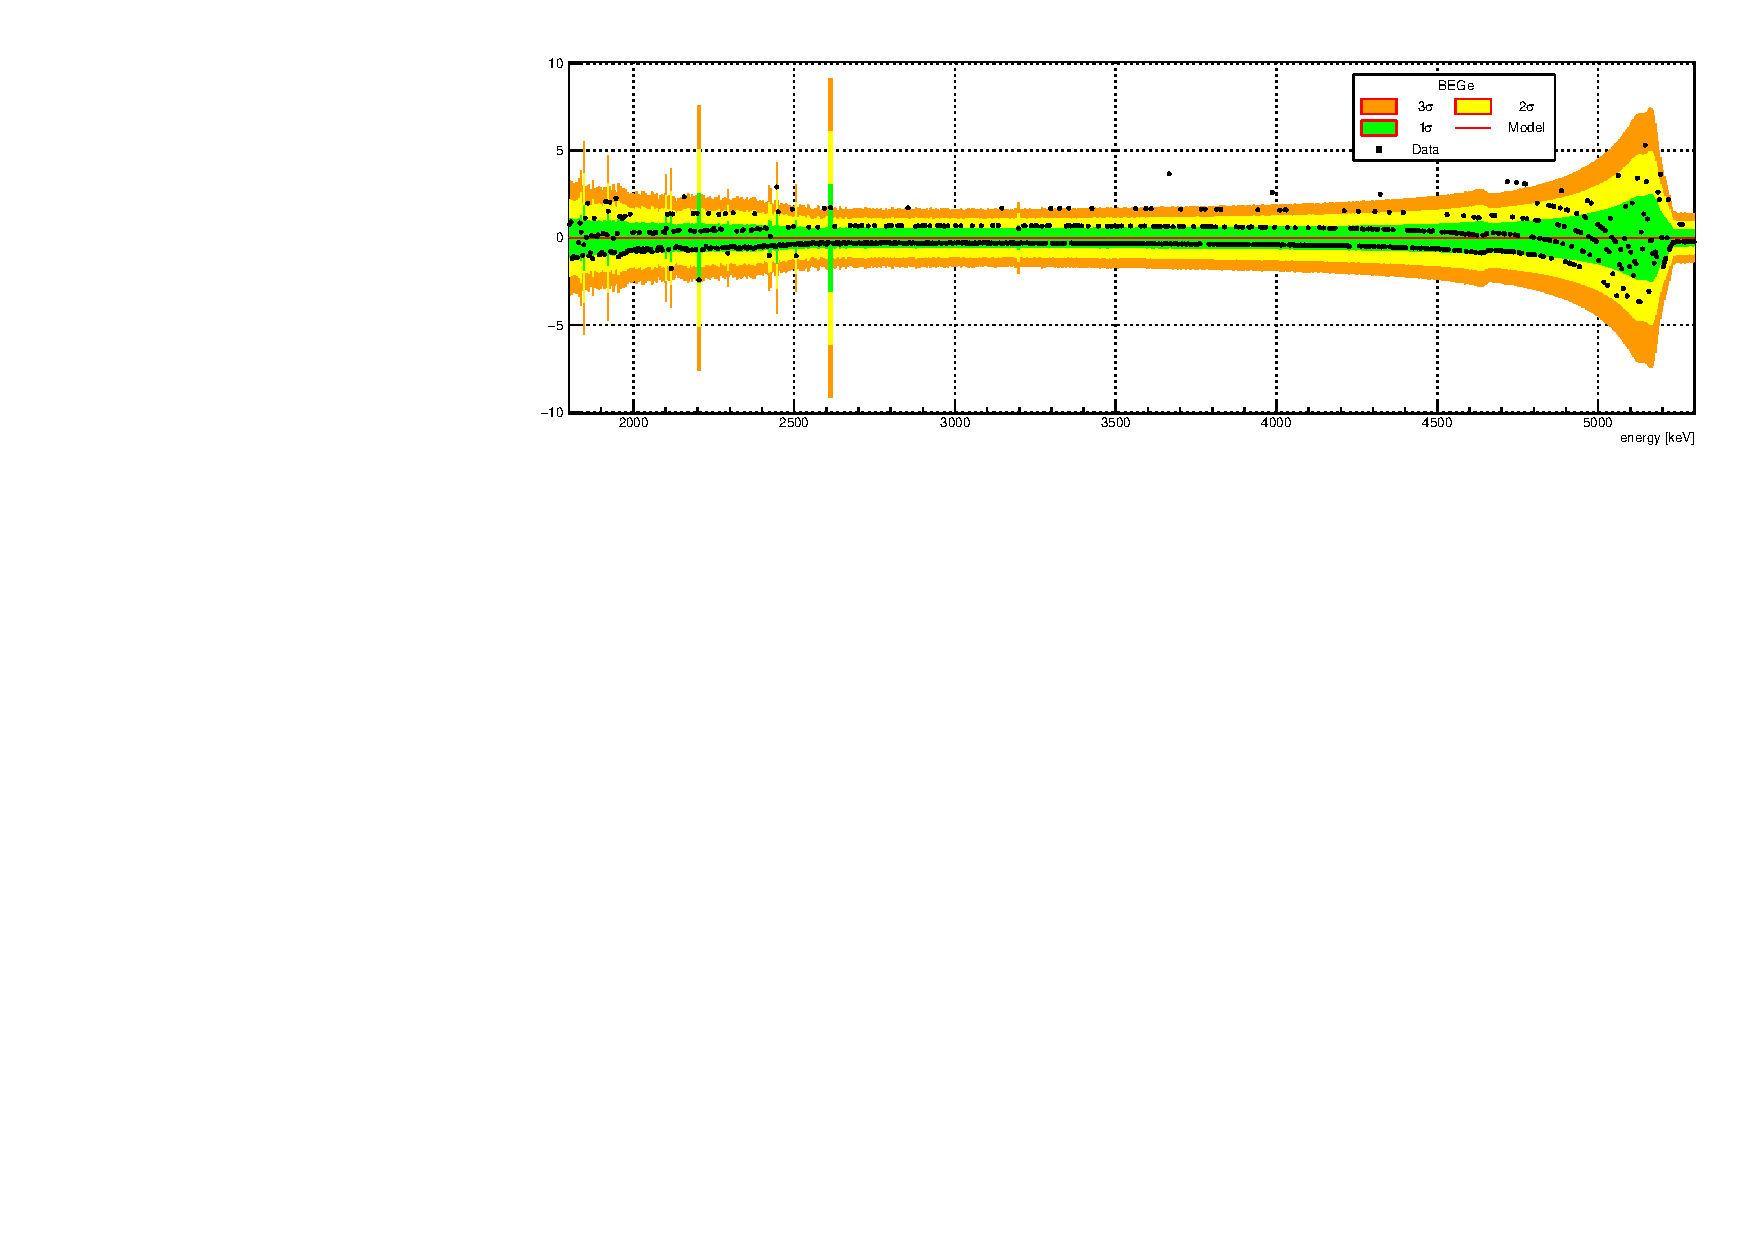
\includegraphics[height=\textwidth, angle=270]{img/resBEGealpha.pdf} \\
	\centering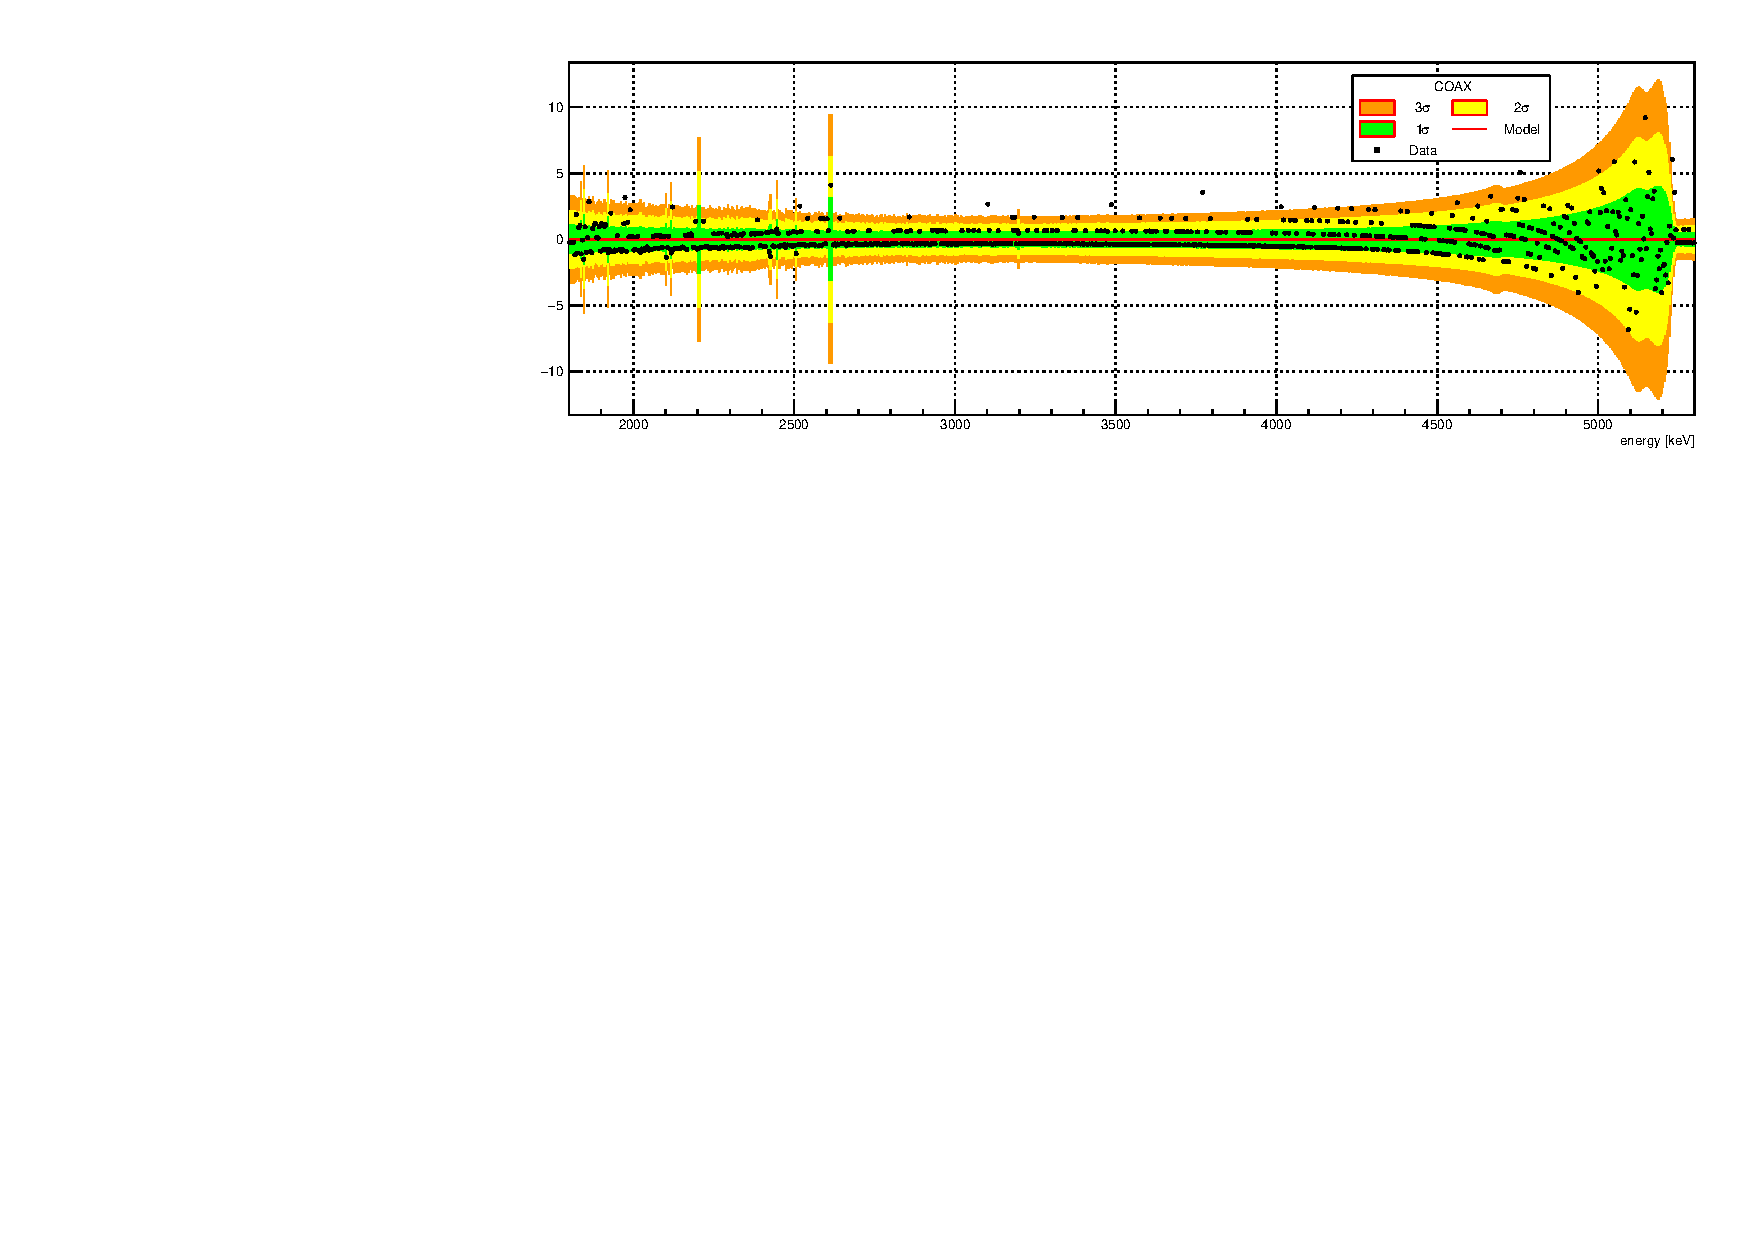
\includegraphics[height=\textwidth, angle=270]{img/resCOAXalpha.pdf}
\end{frame}
\begin{frame}{Results (preliminar!)}
	\begin{itemize}
		\item p-value: $\sim0.3$
	\end{itemize}
	\alert{Some parameters}:
	\begin{itemize}
		\item $2\nbb$ half-life: $1.90\cdot10^{21}$ yr
		\item $\ce{^{42}K}$ in LAr: $1.7\cdot10^{-4}$ Bq/kg
		\item $\ce{^{40}K}$ in fibers: 0.33 Bq/kg
		\item $\ce{^{228}Ac}$ in holders: $3.1\cdot10^{-4}$ Bq/kg
	\end{itemize}
	\uncover{\alert{Coming soon:}}
	\begin{itemize}
		\item The fit was performed assuming flat priors for all parameters, but existing knowledge on activities can be used to constraint the analysis\ldots
		\item Include data from runs > \texttt{74}
		\item Add the Lorentz violating component
	\end{itemize}
\end{frame}
%\begin{frame}[standout]
%	Thank you!
%\end{frame}
\end{document}
